
\chapter{Background}

\section{History}

The Web has evolved from a collection of static documents connected by hyperlinks into a dynamic, rich, interactive experience
driven by client-side code and aggregation by Web services. The security policy of modern browsers was designed to avoid vulnerabilities in old sites, \
rather than to provide the best abstractions for the newest sites. In this section, we summarize the existing access
control policies and the limitations they place on Web site design.



\subsection{90's to 2010}

The Cookie is a fundemental part of client side sessions, crutial to give users certain types of functionality on the web, they were first developed by John Giannandrea,\
Montulli as an attempt to implement a shopping cart website for the initial Netscape cookie specification in 94'. \
Version 0.9beta of Mosaic Netscape, released on October 13, 1994, supported cookies.\

The first use of cookies (out of the labs) was checking whether visitors to the Netscape website had already visited the site.\
Support for cookies was integrated in Internet Explorer in version 2, released in October 1995.\\

The concept of same-origin policy  \ref{SOP} dates back to Netscape Navigator 2 in 1995. All modern browsers implement some form of the Same-Origin Policy as it is an important security cornerstone.\
are often extended to define roughly compatible security boundaries for other web technologies, such as Microsoft Silverlight, \
Adobe Flash, or Adobe Acrobat, or for mechanisms other than direct DOM manipulation, such as XMLHttpRequest.\\

A script can access its document origin’s remote data store using the XMLHttpRequest object, which issues an asynchronous HTTP request to the remote server.\

XML-HttpRequest is the cornerstone of the AJAX programming, and the birthplace of web 2.0 The concept behind the XMLHttpRequest object was originally created by\
the developers of Outlook Web Access (by Microsoft) for Microsoft Exchange Server 2000.
The Mozilla project developed and implemented an interface called nsIXMLHttpRequest into the Gecko layout engine.
This interface was modeled to work as closely to Microsoft's IXMLHTTPRequest interface as possible.\
Mozilla created a wrapper to use this interface through a JavaScript object which they called XMLHttpRequest.The XMLHttpRequest object was accessible as early\
as Gecko version 0.6 released on December 6 of 2000, but it was not completely functional until as late as version 1.0 of\
Gecko released on June 5, 2002. \\
The XMLHttpRequest object became a de facto standard in other major web clients, implemented in Safari 1.2 released in February 2004, Konqueror\
, Opera 8.0 released in April 2005 and iCab 3.0b352 released in September 2005. This is a typical example of Time-to-standard for the web and how features can become standard from a
single entity shipping it, this is also the case for cookies mentioned earlier.\

The World Wide Web Consortium published a Working Draft specification for the XMLHttpRequest object on April 5, 2006, 
edited by Anne van Kesteren of Opera Software and Dean Jackson of W3C.[17] \
Its goal is "to document a minimum set of interoperable features based on existing implementations, allowing Web developers to use these features without platform-specific code.\
" The last revision to the XMLHttpRequest object specification was on November 19 of 2009, being a last call working draft.\

Microsoft added the XMLHttpRequest object identifier to its scripting languages in Internet Explorer 7.0 released in October 2006.\
With the advent of cross-browser JavaScript libraries such as jQuery and the Prototype JavaScript Framework, developers can invoke \
XMLHttpRequest functionality without coding directly to the API. Prototype provides an asynchronous requester object called Ajax.Request\
that wraps the browser's underlying implementation and provides access to it. jQuery objects represent or wrap elements from the current client-side DOM.\
They all have a .load() method that takes a URI parameter and makes an XMLHttpRequest to that URI, then by default places any returned HTML into the HTML element represented by the jQuery object.\

The W3C has since published another Working Draft specification for the XMLHttpRequest object, "XMLHttpRequest Level 2", on February 25 of 2008.
Level 2 consists of extended functionality to the XMLHttpRequest object, including, but not limited to, progress events, support for cross-site requests,\
and the handling of byte streams.The latest revision of the XMLHttpRequest Level 2 specification is that of 16 August 2011, which is still a working draft.\

\subsection{2010-2015}

As of 5 December 2011, XMLHttpRequest version 2 has been merged into the main XMLHttpRequest specification, and there is no longer a version 1 and a version 2.\

Of course initially AJAX had to also follow the SOP, today’s browser abstractions offer an all-or-nothing trust model for Web programmers. \
Site a.com either does not trust Site b.com ’s content at all by segregating b.com ’s content into a frame or a.com trusts b.com ’s scripts\
entirely by embedding b.com ’s scripts and giving them full access to a.com ’s resources.\

In order to provide more fine grained handling of access origin inlight of web 2.0 application the rigidness of SOP was aleviated through the Cross Origin Resource Sharing Policy.\
Proposed by Matt Oshry, Brad Porter, and Michael Bodell of Tellme Networks in March 2004 for inclusion in VoiceXML 2.1 to allow safe cross-origin data requests by VoiceXML browsers.\
The mechanism was deemed general in nature and not specific to VoiceXML and was subsequently separated into an implementation NOTE.\
The WebApps Working Group of the W3C with participation from the major browser vendors began to formalize the NOTE into a W3C Working Draft on track toward formal W3C Recommendation status.\\

The Content Security Policy is a more recent developement that sought to provide web designers or server administrators with much more fine grained control \
over how content interacts on their web sites.It helps mitigate and detect types of attacks such as XSS and data injection more directly . \
CSP is not intended to be a main line of defense, but rather one of the many layers of security that can be employed to help secure a web site.\

at the time BrowserAudit was made the latest draft of CSP1.1 released in June 2014 was the latest and was not an \
official Recommendation or RFC. We have now reached Level 2 policy as of 19'th of February,\cite{csp} this is a candidate Recommendation.\

Note the attachement to precise terminology regarding the specification of the main subjects of interest of this paper. This is because this\ 
paper is largely an integration project that requires an in-depth insight of the direction of the standards in order to be able to prioritise features to be added to BrowserAudit2.0\

\section{High level overview of browser functions}

In this section we will go through an intuitive view of how a vanilla browser would function.\

The browser communicates with the server by making HTTP requests. we will briefly describe HTTP 1.1\
after going through the request format which is the browser convention this format based on URLs \
is later converted appropriately to HTTP requests and we will see that the particulars affect \
security behaviour of the browser.\

\subsection{Uniform Resource Locators}

A uniform resource locator (URL) identifes a specifc resource on a remote server. Com-\
monly referred to as a web address, it is usually displayed prominently in a web browser's\
user interface. The URL syntax is detailed in \cite{URL}; there are many optional\
elements, but a good working example is as follows:\\

\begin{verbatim}
scheme://host:port/path?query_string#fragment
\end{verbatim}

The schemes, otherwise referred to as protocols, used most commonly by web applications
are http:and https:. Other examples of schemes are ftp: and file:, and pseudo-URLs that begin with
data: and javascript:.\
The host is most commonly a domain name (e.g.example.com) but can also be a literal
IPv4 or IPv6 address. If not otherwise specifed, the port defaults to the port associated
with the scheme (80 for http: and 443 for https:).\\

The path is used to specify the resource being accessed. The query string parameters
contain optional data to be passed to the software running on the server. The fragment
identifer, also optional, specifes an exact location within the document. In HTML
documents, these fragment IDs are often combined with anchor tags to allow hyperlinks
to specifc sections within a document.\
The most important elements of a URL as far as we are concerned are the scheme, host
and port. We have mentioned them but will see later in more details that, together as a tuple, they form a concept known as
an origin used in many browser security concepts.\\

\subsection{What is HTTP/1.1?}

\begin{verbatim}
FROM THE RFC:

HTTP 1.1

   The Hypertext Transfer Protocol (HTTP) is an application-level
   protocol for distributed, collaborative, hypermedia information
   systems. It is a generic, stateless, protocol which can be used for
   many tasks beyond its use for hypertext, such as name servers and
   distributed object management systems, through extension of its
   request methods, error codes and headers. A feature of HTTP is
   the typing and negotiation of data representation, allowing systems
   to be built independently of the data being transferred.
   HTTP has been in use by the World-Wide Web global information
   initiative since 1990. This specification defines the protocol
   referred to as "HTTP/1.1", and is an update to RFC 2068.
  
\end{verbatim}
 
Version 1.1 adds a couple of features compared to 1.0 regarding connection type like the chunked and keep open options.\
It also has better caching support with vary and cache-control and etags .There is a new HTTP method OPTIONS which is typically used for CORS.\
few new status codes better compression and authentication and other network and security improvement and is a lot more extensible.\\
  
\subsection{what about HTTPS/TLS?}

This is nothing more than HTTP/1.1 tunnelled through a TLS socket which is the improvement on SSL\
this means that traffic is much more safe from eavesdropping on the line, otherwise called man-in-the-middle attacks\
and means integrity properties can be met as well. How good the crypto implementation is a direction we could take\
but we're not too certain at the moment we will just give this a passing mention.\\

\subsection{Basic interaction, request and response}

The HTTP verbs we care about the most for this paper are the GET and POST methods, these have near identical syntax for requests\
and slight differences in responses, and the proper semantics is supposed to be that GET is used to fetch content and POST for\
initiating action on the server, perhaps also meaning fetching content, although with AJAX this has changed slightly they roughly\
do the same thing, except GET requests are more cacheable, bookmarkeable etc.. and is easier to tamper with, there is a natural ease\
to use POST requests for uploading or dealing with forms because that is the most commonly held use of it and the browser developer intent\
behind it.\ Two other distinctions to keep in mind between these two HTTP verbs is that in GET requests parameters are serialised in the parameter\
and hence have a much smaller length (7607 characters) whereas POST requests passes the parameters in the body of the requests making the limit of 8Mb, and offers more marshalling formats.\
This have repercussions on the security of GET requests and in particular for opening the attack tree for CSRF attacks see \ref{subsec:CSRF}.\
an example request header:\\

\begin{verbatim}
GET / HTTP/1.1
Host: www.duckduckgo.com/
Connection: close
User-Agent: Web-sniffer/1.1.0 (+http://web-sniffer.net/)
Accept-Encoding: gzip[CRLF]
Accept-Charset: ISO-8859-1,UTF-8;q=0.7,*;q=0.7
Cache-Control: no-cache[CRLF]
Accept-Language: de,en;q=0.7,en-us;q=0.3
Referer: http://web-sniffer.net/
\end{verbatim}

and the corresponding response header:

\begin{verbatim}
 -- response --
200 OK
Server:  nginx
Date:  Tue, 24 Feb 2015 21:23:21 GMT
Content-Type:  text/html; charset=UTF-8
Expires:  Tue, 24 Feb 2015 21:23:20 GMT
Cache-Control:  no-cache
Strict-Transport-Security:  max-age=31536000
Content-Encoding:  gzip
X-Firefox-Spdy:  3.1
\end{verbatim}

The two have similar structure which is a column seperated name value pair, these are called HTTP fields \
and they allow to negotiate the parameters for acceptable encoding and compression of data back and forth \
among other things like caching, cookies etc.. \
The request is followed by a response of course, except when a http HEAD request is made, often to test if a resource or website is live.\\

\subsection{Important header verbs and fields}

the most important request header are the first line, Host and User-Agent.. For our purposes it is also important \
to look at the Refer header, which is problematic for privacy but also allows to warn against wandering off a \
trusted HTTPS connection ..\\

The tables in \ref{tab:req}, \ref{tab:resp} present the main headers we're interested in with a brief description for HTTP requests and responses correspondingly.\

\begin{table}
\centering
\begin{tabular}{p{2cm}|p{6cm}|p{4cm}|p{2cm}}
Header name & Description & Example & Status \\\hline

Cookie & An HTTP cookie previously sent by the server with Set-Cookie (below) & Cookie:\$Version=1; Skin=new; & permanent \\
Origin &Initiates a request for cross-origin resource sharing (asks server for an 'Access-Control-Allow-Origin' response field) . & Origin: http://www.example-social-network.com & Permanent: standard\\
Referer [sic] & This is the address of the previous web page from which a link to the currently requested page was followed. & Referer: http://web-sniffer.net/ & Permanent\\
User-Agent & The user agent string of the user agent & User-Agent: Mozilla\/5.0 (X11; Linux x86\_64; rv:12.0) Gecko/20100101 Firefox/21.0 &Permanent
\end{tabular}
\caption{\label{tab:req}List of request headers of interest to this paper.}
\end{table}


\begin{table}[H]
\centering
\begin{tabular}{p{2cm}|p{6cm}|p{4cm}|p{2cm}}
Header name & Description & Example & Status \\\hline
Set-Cookie &	An HTTP cookie 	Set-Cookie: UserID=JohnDoe; Max-Age=3600; Version=1 &Permanent: standard\\
Status &CGI header field specifying the status of the HTTP response. &	Status: 200 OK 	& Not listed as a registered field name\\
Strict-Transport-Security & A HSTS Policy informing the HTTP client how long to cache the HTTPS only policy and whether this applies to subdomains. &Strict-Transport-Security: max-age=16070400; includeSubDomains &Permanent: standard\\
X-Frame-Options[34] &Clickjacking protection: deny - no rendering within a frame, sameorigin - no rendering if origin mismatch, allow-from - allow from specified location, allowall - non-standard, allow from any location[35] &X-Frame-Options: deny &Obsolete\\
X-XSS-Protection[39] &Cross-site scripting (XSS) filter &X-XSS-Protection: 1; mode=block& non-standard \\
Content-Security-Policy &X-Content-Security-Policy X-WebKit-CSP Content Security Policy definition& X-WebKit-CSP: default-src 'self' & Working draft
\end{tabular}
\caption{\label{tab:resp}List of response headers of interest to this paper}
\end{table}

\subsubsection{Cookies}
\label{cookie}
Cookies are set through responses by the Set-Cookie command, and has always been the only way to get state in a stateless protocol such as http \
Cookies are sent with every subsequent request to the same domain. This meant that through the years developers added attributes to cookies \
to enhance security.\
the HTTPonly attribute mandates to the browser is only accesible through the Http request and not through the client side, making it impossible \
to steal the cookie directly after an XSS attack.\
There is also the Secure attribute, which ensures that the cookie is only included if HTTPS is used.\\

Cookies are set by the server through set-cookie headers that look a little like this: \
\begin{verbatim}
 Set-cookie: name = value; [(attribute [= value];)*]
\end{verbatim}

and as we said sent in subsequent requests but there is a bit more to it:
\begin{itemize}
 \item the cookies are scoped by the origin of the server.\
 \item Cookie origin:domain,path.\
 \item Cookie is identified by name and origin.\
 \item Cookie  scope is	determined  by origin and secure attribute.\
 \item Browser request sends all cookies that are in scope to server.\
 \item The attributes are not sent back in the requests so server cannot know if cookie is httpOnly, set in Subdomain or by javascript.\
 \item SOP allows elements in the same path to see cookies (as illustrating in the next Origins section).\
 \item Even secure attribute does not guarantee cookie integrite , as we see in XST section \ref{label:xst} 
\end{itemize}

\subsection{Origins}

An origin is defined as a combination of URI scheme, hostname, and port number.
For examples ,all of the following resources have the same origin:
   http://example.com/
   http://example.com:80/
   http://example.com/path/file

   Each of the URIs has the same scheme, host, and port components.

   Each of the following resources has a different origin from the
   others.

   http://example.com/
   http://example.com:8080/
   http://www.example.com/
   https://example.com:80/
   https://example.com/
   http://example.org/
   http://ietf.org/

   In each case, at least one of the scheme, host, and port component
   will differ from the others in the list.

Origins are required to implemet Same Origin Policy and as explained is the most rudimentary client side security mechanism.
 
\subsection{the DOM, javascript and CSS}

\textbf{The Document Object Model}
The document object model is a specially connected tree of DOM elements , representing the structure \
of the HTML page which has an xml like semantics. Different types of tags have different display features \
on the browser and different default styling and animation behaviour. The DOM also allows the creation of \
script tags that point to scripts to be fetched and executed in the scope of the document as well as stylesheet \
nodes. Modern browsers add many utility and other things on top of the DOM.

\textbf{Javascript}
Javascript is the scripting language that is shipped with browsers nowadays, It is a weakly typed dynamic functional \
programming language with prototypical inheritence, it was developed by Brendan Eich in 11 days at Netscape. Stressing \
the point that in the web often things get made very quickly to match competition or attract market and these things \
are sometimes not temporary. which might be a problem for security.

Javascript is in it's 6th iteration though and glaring security issues can be avoided if enough care is taken \
Javascript is passed to the browser in UTF-16 format and is immediately parsed and code starts to run asap \ 
usually hooking into the document.load or document.ready event and there are many libraries that support \
module pattern and asynchronous loading used nowadays\\

The quick parsing and the permissive semantics of javascript means there are possibilities of serious security \
flaws, the most prominent of which relate to the ability to evaluate scripts inside scripts which is heavily \
discouraged but has limited valid applications.\\

\textbf{CSS}

Cascading stylesheets are a way of providing styling directives to the browser and is composed of the set of attributes \
exposed explicitely though the 'style' attribute of a DOM element and a selector language that can have classes , identifiers \
that are also DOM based and pseudo-selectors which are CSS specific. \
There are also possibilities of leakage due to the fact that the browser has to parse these and apply the values to the document \
sometimes not in the most secure way for the user.\\

\subsection{XMLHTTPRequest}

this API allows to make requests to any server after a page have been loaded from a server. As explained lengthily in the History section.\
this is the underlying primitive of web 2.0 applications. Which loads resources on the fly usually from many domains and is typically invoked using\
an AJAX call in Jquery or other basic library that programmers use.

for example this code that saves some code to server  and notifies the user of the response when complete.
\begin{verbatim}
$.ajax({
type: "POST",
url: "some.php",
data: { name: "John", location: "Boston" }
})
.done(function( msg ) {
alert( "Data Saved: " + msg );
});\end{verbatim}

We will restate here that this is the main driver for Cross Origin Resource Sharing policy and opens up the attack surface drastically. because \
requests can be made sometimes undetected after a page is loaded when a script is injected or made to run somehow with the right Origin.\

\subsection{external objects}

In order to have extra functionality and circumvent limitations of the browser, we have to rely on external objects that can be bundled \
through browser Object objects or other special tags, notable examples of these is Flash Objects or Java applets

\section{Attacks on the client}

\subsection{XSS}


Cross site scripting attacks refers to any way of getting javascript or other code running on your browser within the domain \
originating from the server you're accessing such that it's not in violation of the same origin policy.\
This essentially means that they abuse the trust you have for a particular website in order to run malicious code as if originating\
from the site\
This can be done in a number of ways, there are three main classes of XSS attacks that span the possibilities.\\

\textbf{Reflected XSS attacks}

These account for 75\% of XSS attacks also called first order XSS they work by abusing the fact that in certain websites\
developers create a unified error message function which prints back the error from a field in the URL\
This allows the malicious user to input a payload in an error page by supplying the URL to the user somehow and have the payload executed.\
The more general working can be seen in \ref{fig:xssref}. Of course the payload can do further things like steal the cookie etc..\

\begin{figure}
\centering
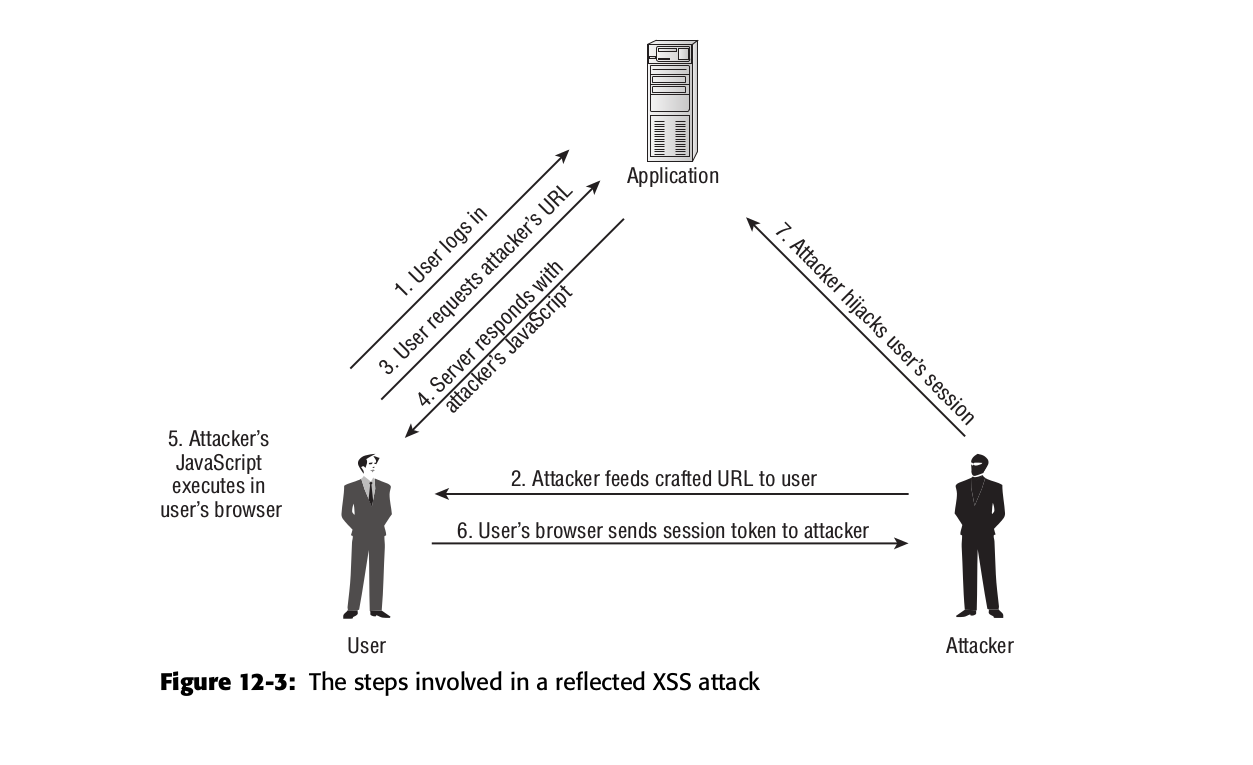
\includegraphics[width=1\textwidth]{refl-XSS.png}
\caption{\label{fig:xssref}steps involved in reflected XSS attack}
\end{figure}

\textbf{Stored xss attacks}

In the stored variant of an XSS attack the principle is similar, but the mechanism of getting the code to run relies on any part\
of the website that stores arbitrary content without proper sanitasation and then renders it to users on the site\
this is a very common threat is social media sites or other side with aggregation of user generated content.\\
see \ref{fig:xsssto} this is also called a second order XSS attack. They can be in-band meaning generated through some input on the web\
application itself. or out of band meaning through some other path to the database or backend holding the data.\

\begin{figure}
\centering
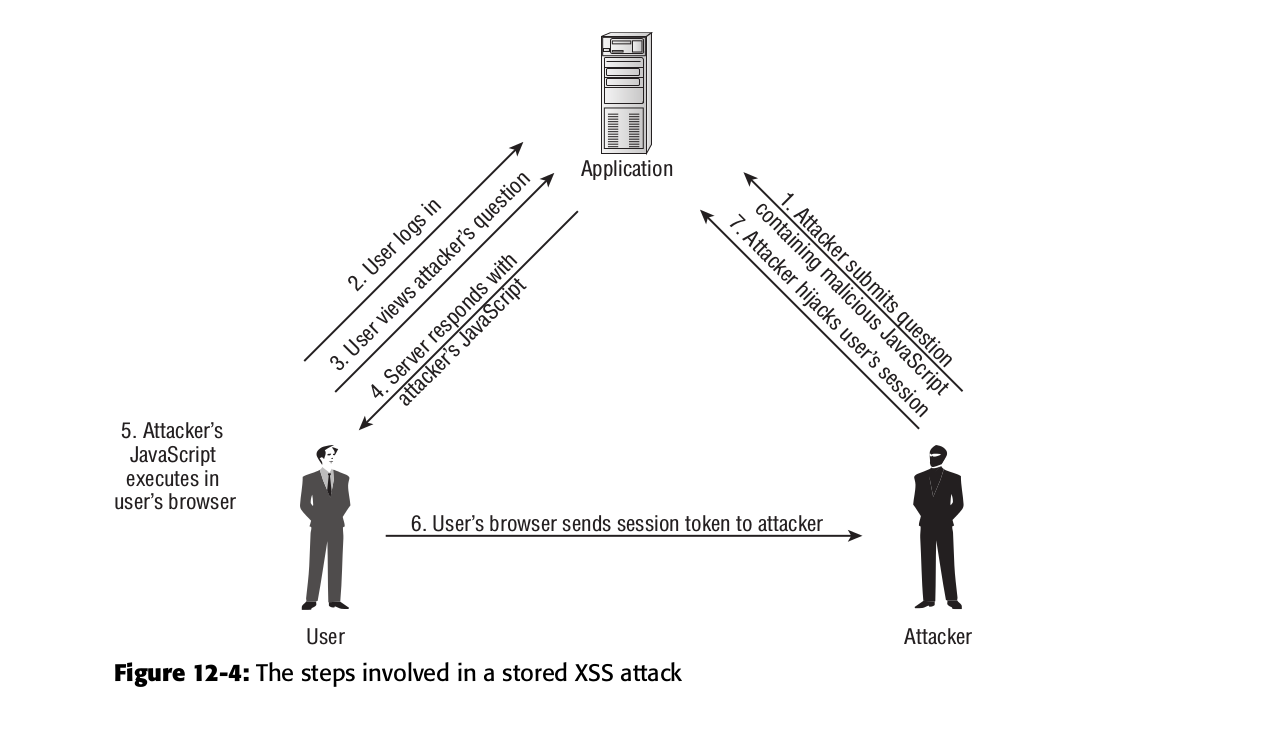
\includegraphics[width=1\textwidth]{stored-XSS.png}
\caption{\label{fig:xsssto}steps involved in stored XSS attack}
\end{figure}

\textbf{DOM based XSS attacks}

The DOM based variant is similar to the reflected XSS bug in that it requires the user to visit a crafted url.\
the difference is that it relies on server processing or already existing Javascript code that automatically runs\
that turns the crafted url into malicious javascript that gets loaded.\
As you can imagine this means that the attacker conducts a phase of careful investigation of the server processing of url\
content as well as scripts that are loaded with the page by default.\\

\begin{figure}
\centering
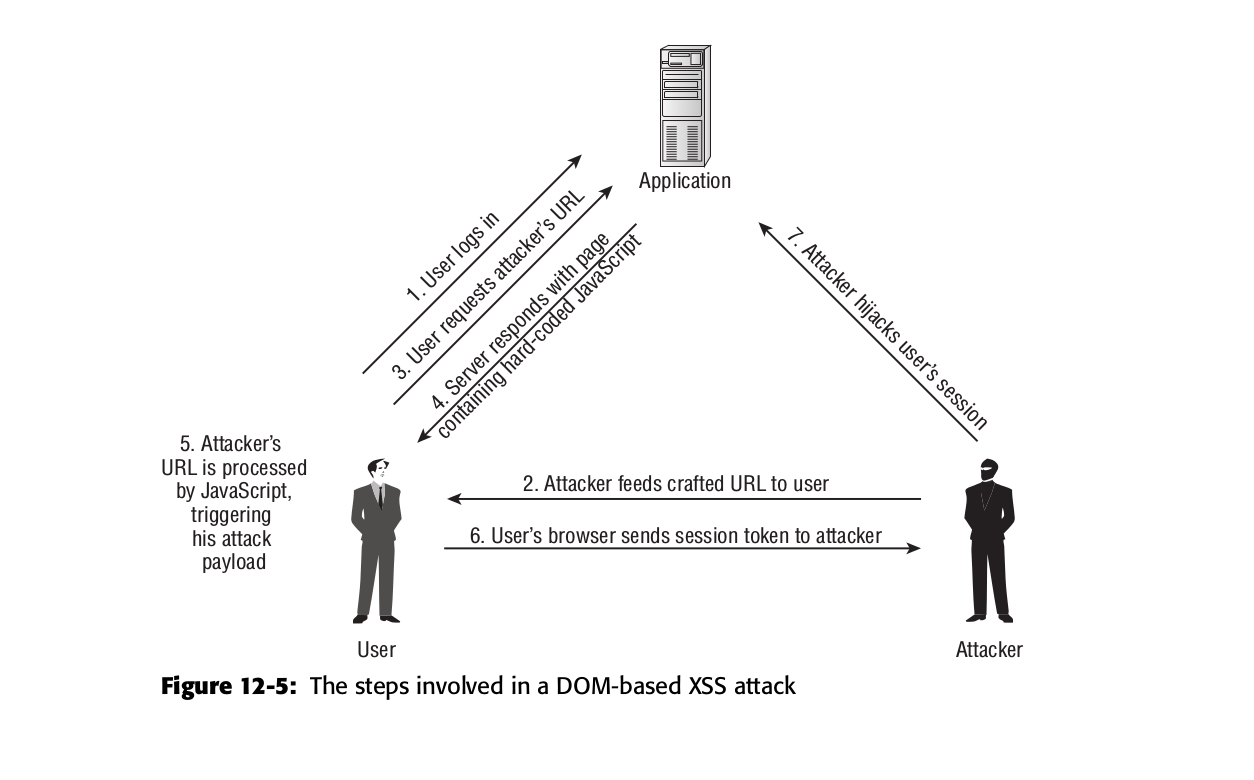
\includegraphics[width=1\textwidth]{DOM-XSS.png}
\caption{\label{fig:xssdom}steps involved in DOM based XSS attack}
\end{figure}

\emph{brief discussion of XSS}

Reflected and stored XSS have two important differences in the attack process. Stored XSS generally is more serious from a security perspective.

First, in the case of reflected XSS, to exploit a vulnerability, the attacker must induce victims to visit his crafted URL.\
In the case of stored XSS, this requirement is avoided. Having deployed his attack within the application, the attacker \
simply needs to wait for victims to browse to the page or function that has been compromised.\
Usually this is a regular page of the application that normal users will access of their own accord.\

Beyond the scope of preventing 'attacks to other users' and potentially nasty consequences for the web applications in terms of gaining admin. privileges \
and performing other attacks but another topical issue entailed by this attack vectors is stealing data. \
There has been a rise in the appetite for accurate data and techniques such as preventing cookies have had very small impact of advertisers potential \
for obtaining the data about users due to mechanisms such as super-cookies or fingerprinting. \

There is also high social and disruption cost by certain types of XSS defacement attacks especially when combined with worm like behaviour.\

We will note that the major reason why XSS is overlooked is that it doesn't offer the most precise way of targeting users or websites. often hackers\
prefer to opt for the more direct flaws which are ever-growing on the server or on the network to have more full control. Nevertheless in certain circumstances\
and if a hacker's purpose is not specific targeting XSS is a very reasonable approach that can yield great results and can allow a hacker to completely compromise\
an unprotected web application.\ 

Typically mitigation is done through either reducing the risk of stealing the cookie (http-only , secure) or using some encrypted local store. As well as writting\
complicated Regular expression or evaluation based filters that sanitises inputs and parameters either through whitelist or blacklist ensures code does not leak into the \
origin and manage to run. \
The CSP policy can help drastically with this by restricting the script-src to disallow code to run from any remote origin, see CSRF \ref{label:CSP}.\\

\subsection{CSRF}
\label{subsec:crsf}

Unlike XSS which abuses your trust for a particular domain, Cross Site Request Forgery abuses your trust for the browser.\
What we mean by this is that CSRF relies on the fact that you are connected and have the cookie to a particular site that the hacker wants to attack.\
often for sites like facebook or google this is a reasonable assumptions since people leave them on when they go about their browsing.\ Then suffice it for the user
to point to a domain where a hidden form has been injected or that is under the control of the hacker. \
he can perform unauthorised actions to the web application targeted abusing the fact that the browser will send the cookies as if authenticated.\
This is a serious threat, but relies on both having a good map of the functions of the target application and that the user is authenticated to the particular account you are\
targeting which is not of particular concern to sites where users are not often connected.\

These kind of attacks came in these main flavours:

\subsubsection{Session CSRF}

\begin{figure}
\centering
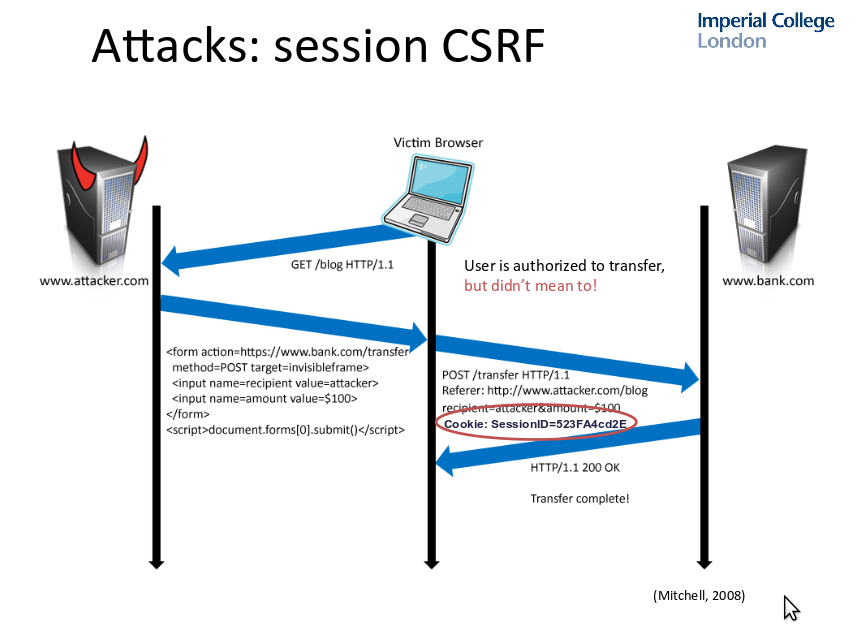
\includegraphics[width=1\textwidth]{./sessioncsrf.png}
\caption{\label{fig:sessioncsrf}The typical session Cross Site Request Forgery}	
\end{figure}


The most common case is simply to somehow inject a hidden frame by tricking the user to your attack site (through deception or some kind of DNS poisoning)
that performs a form submission using the token you had already authenticated hence causing you to perform an unwanted action\ Check \ref{fig:sessioncsrf}
for illustration.

\subsubsection{Login CSRF}

\begin{figure}
\centering
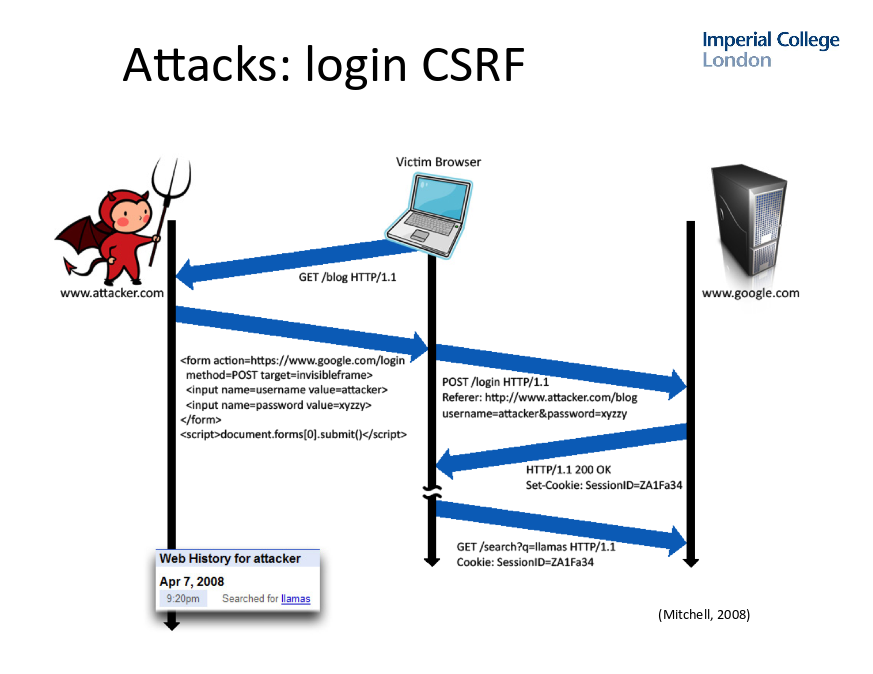
\includegraphics[width=1\textwidth]{./logincsrf.png}
\caption{\label{fig:logincsrf}The login Cross Site Request Forgery let's attacker abuse interconnectivity of Google services}
\end{figure}

This is an interesting variant, whose payload is a frame that authenticates the attacker's credentials to a service that the unknowing user uses, in that way exploiting
the internal cohesion provided by Google for example, To get reports of the user's google search history on your interface. Check \ref{fig:logincsrf}
for illustration.

\subsubsection{Redirection CSRF attack}


Where an attacker exploits flaws in certain designs where redirection is somehow parameterised and exploits tools like facebook connect which is used by many sites .
Instead of redirecting the facebook token to the desired site for example yahoo.com it uses a yahoo internal server logic and queries yahoo.com/redirect?attacker.com to exploit
the token from the attacker site.



\subsubsection{Social CSRF}

\begin{figure}[H]
\centering
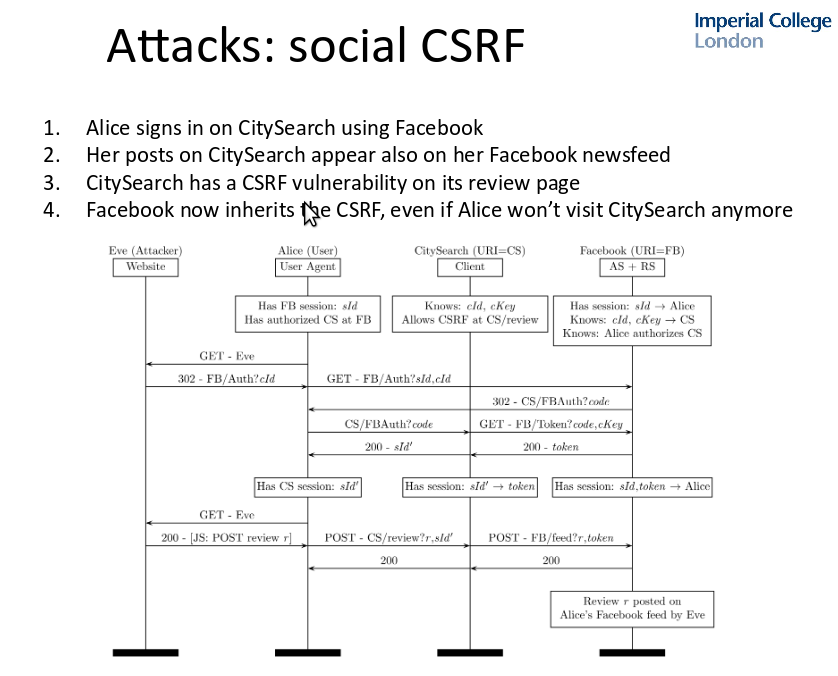
\includegraphics[width=1\textwidth]{./socialcsrf.png}
\caption{\label{fig:socialcsrf}The Social csrf : discoverd through automated reasoning tools }
\end{figure}
This happens in the case of an affiliate service like CitySearch on facebook, 
The mechanism is that you are redirected from the attacker site to login to a service like facebook. And then since the affiliate could have a csrf vulnerability \
you abuse the vulnerability to propagate the csrf through facebook, in a sense exploiting not only the trust of the browser in facebook but the permissions granted by the \
trust between the affiliate and facebook. Check \ref{fig:socialcsrf} for illustration.

\subsubsection{More about CSRF}

Remember that by using the GET methods where some of the above attacks, when it let's the user be redirected from the target site to your site allow to leak POST parameters through the 
refer header, the header that shows where you've been last , used mainly for advertisers and affiliate programs. This one of the reasons why POST is more secure in forms.

Note that there are also other possibilities of abuse, where for example a compromised machine has access to network services in the LAN, in which a CSRF would allow abuse
of this privilege , but we do not go more in depth into this because our focus is the browser we will only cite the csrf soho router attack : \cite{soho}.

These attacks are typically mitigated through use of csrf tokens in forms, which could be putting the very cookie as a form field or more securely a different token, usually the \
hash of the session and the desired action or something of the kind.\ Except in some edge cases like social csrf or redirection attack using the CSP policy connect-src directive would also block the attacker.
from posting forms to sites that your site does not normally contact.\\

\subsection{XST}
\label{label:xst}

We mentioned earlier in the cookie section that one way of mitigated the XSS attack is to use HTTP only cookie options.\
there are unfortunately a way around this with Cross Site Tracing, which uses the diagnostic HTTP trace method in a manner that allows it\
to retrieve the HTTP only cookie. If the cookie is secure as well (meaning encrypted) the chances become slim of obtaining the cookie.\


\subsection{Framebusting or clickjacking}

These attacks are especially pervasive in the top websites. and consist in tricking the users into clicking on the content of another site\
which is placed in a visibility:hidden Iframe behind the current highlighted content. This is the reason for a Chrome and Firefox X-frame-Options\
header. see \cite{buster} for many real life example with twitter for example.

\subsection{Other}

Another overall privacy aware security policy in the browser is Refer Header (which is also source of XSS attacks potentially) and proposed HSTS mechanism \
we will evaluate effectiveness of those mechanisms and will see through that a compliant web browser which passes BrowserAudit could be made to minimze \
information leakage, of course the mechanisms that law enforcement (and criminals alike) might use on lower levels of the networking stack are outside the scope of this paper.\
We will also note that openSSL and WebCrypto implementation of the browser was not tested by BrowserAudit tool.\


\section{Security policies}

\subsection{Same Origin Policy}

\label{label:SOP}
(SOP) governs the access control on today’s browsers. The SOP prevents documents or scripts loaded from one origin from getting or setting properties of documents \
from a different origin . (The origin that a script is loaded is the origin of the document that contains the script rather than the origin that hosts the script.) \
Two pages have the same origin if the protocol, port (if given), and host are the same for both pages.

Each document is associated with an origin. The SOP policy concerns three browser resources: cookies, the HTML document tree, and remote store access.\
In more detail, a site can only sets its own cookie and a cookie is sent to only the site that sets the cookie along with HTTP requests to that site.\
Two documents from different origins cannot access each other’s HTML document using the Document Object Model (DOM) which is a platform- and language-neutral\
interface that will allow programs and scripts to dynamically access and update the content, structure and style of documents.\\


\subsection{Cross Origin Resource Sharing}
\label{label:CORS}

As seen in te previous section User agents commonly apply same-origin restrictions to network requests. These restrictions prevent a client-side Web application\
running from one origin from obtaining data retrieved from another origin, and also limit unsafe HTTP requests that can be automatically\
launched toward destinations that differ from the running application's origin.\\

In user agents that follow this pattern, network requests typically include user credentials with cross-origin requests, including HTTP authentication and cookie information.

We mentioned in the history section that CORS extends SOP and it extends this model in several ways:

A response can include an Access-Control-Allow-Origin header, with the origin of where the request originated from as the value, to allow access to the resource's contents.\
The user agent validates that the value and origin of where the request originated match.\
User agents can discover via a preflight request whether a cross-origin resource is prepared to accept requests, using a non-simple method, from a given origin.\
This is again validated by the user agent.\\

Server-side applications are enabled to discover that an HTTP request was deemed a cross-origin request by the user agent, through the Origin header.\
This extension enables server-side applications to enforce limitations (e.g. returning nothing) on the cross-origin requests that they are willing to service.\
This specification is a building block for other specifications, so-called CORS API specifications, which define how this specification is used.\\
Examples are Server-Sent Events and XMLHttpRequest. [EVENTSOURCE] [XHR]

If a resource author has a simple text resource residing at http://example.com/hello which contains the string "Hello World!" \
and would like http://hello-world.example to be able to access it, the response combined with a header introduced by this specification could look as follows:\

Access-Control-Allow-Origin: http://hello-world.example\\

Hello World!\\

Using XMLHttpRequest a client-side Web application on http://hello-world.example can access this resource as follows:\\
\begin{verbatim}

var client = new XMLHttpRequest()
client.open("GET", "http://example.com/hello")
client.onreadystatechange = function() { /* do something */ }
client.send()
 
\end{verbatim}

It gets slightly more complicated if the resource author wants to be able to handle cross-origin requests using methods other than simple methods.\
In that case the author needs to reply to a preflight request that uses the OPTIONS method and then needs to handle the actual request that uses \
the desired method (DELETE in this example) and give an appropriate response. The response to the preflight request could have the following headers specified:\\

\begin{verbatim}

Access-Control-Allow-Origin: http://hello-world.example\
Access-Control-Max-Age: 3628800\
Access-Control-Allow-Methods: PUT, DELETE\
 
\end{verbatim}

The Access-Control-Max-Age header indicates how long the response can be cached, so that for subsequent requests, within the specified time, \
no preflight request has to be made. The Access-Control-Allow-Methods header indicates the methods that can be used in the actual request.\
The response to the actual request can simply contain this header:\\

\begin{verbatim}
Access-Control-Allow-Origin: http://hello-world.example 
\end{verbatim}

The complexity of invoking the additional preflight request is the task of the user agent. Using XMLHttpRequest again and assuming the \
application were hosted at http://calendar.example/app the author could use the following ECMAScript snippet:\\

\begin{verbatim}

function deleteItem(itemId, updateUI) {
  var client = new XMLHttpRequest()
  client.open("DELETE", "http://calendar.example/app")
  client.onload = updateUI
  client.onerror = updateUI
  client.onabort = updateUI
  client.send("id=" + itemId)
} 
\end{verbatim}

\subsection{Content security Policy}
\label{label:CSP}

The content security policy  is the modern solution to the previous mess of SOP and CORS. It is a clean specification loaded with a page\
as a meta attribute or via an HTTP header.\
It allows to define custom made policies that specify which origins are allowed PER HTML entity/tag. meaning that one can say that scripts can only come\
from a particular set of domains and images from another. when used properly this hugely decreases the risk of CSRF, clickjacking or frambusting.\

To mitigate XSS attacks, for example, a web application can declare that it only expects to load script from specific, trusted sources.\
This declaration allows the client to detect and block malicious scripts injected into the application by an attacker. check \cite{csp} for latest standard.\
DOM based XSS is still possible in some cases.\\

an example policy delivered in meta tag is 
\begin{verbatim}
 <meta http-equiv="Content-Security-Policy" content="script-src 'self'">
\end{verbatim}

Multiple policies can be enforced which means that the most restrictive rules are applied example in the document containing both these policies.\
\begin{verbatim}
Content-Security-Policy: default-src 'self' http://eg.com http://example.net;
                         connect-src 'none';
Content-Security-Policy: connect-src http://eg.com/;
                         script-src http://eg.com/
\end{verbatim}

we cannot connect to http://eg.com because of the connect-src 'none'; rule.
The Standard has report uri facility which allows to flag and report security violations to be sent to a defined URL.

\begin{verbatim}
 Content-Security-Policy-Report-Only: script-src 'self';
                                     report-uri /csp-report-endpoint/
\end{verbatim}

There is also another feature highlighted in this example which is the possibility of only reporting CSP violations. which could be a first line for iteratively\
defining the suitable policy for a web application that might not be aware of all the components he is using in modern web applications. Or that might find offending\
behaviour that needs to be studied first before enforcing the policy.\\


\subsection{X-frame-Options}
\label{X-frame-Options}
Mentioned earlier this specifies which Origin is allowed to render the document in a frame. this can apply to <frame>, <object>, <applet> and <embed> elements.\
The options available for Origin are DENY , SAMEORIGIN, or ALLOW-FROM and this feature is supported in most modern browsers.\
It would certainly make a lot of streaming websites less annoying if they used this header but Perhaps also less lucrative,in the common case of ad clickjacking.\

\subsection{HSTS}

HSTS defines a mechanism enabling web sites to declare themselves accessible only via secure connections and/or for users to\
be able to direct their user agent(s) to interact with given sites only over secure connections. The policy is declared by web\
sites via the Strict-Transport-Security HTTP response header field and/or by other means, such as user agent configuration, for example.\\

\section{Adoption}

We felt that the common plague of security in technology in general is relevant here as well, information about the security while widely \
available requires substantial effort for a novice or even seasoned developer to understand since the standards keep changing and browsers \
differ on priorities at the moment. There is also a need for more usability and for developers to know easily which server options to use \
to perhaps make it less frustrating and time consuming like setting up a new 

There are also many subtle ways in which trust boundaries can be exploited and it's useful to think about how much more trust you have for libraries and mashups you allow in your site.\
and we cannot seperate. and often cases making a more lenient but robust security mechanism can mean the world. Because Hackers do not get frustrated with a certain restriction;\
and end up doing something silly from a security perspective like putting a foreign untested script within your trusted scripts or randomly adding any domain to your CORS.
We will need to acquire data about vulnerable browsers and adoption figures with things such as common policies, this is particularily hard to find and will be an objective of ours.\

